\begin{figure*}[!t]
    \centering
    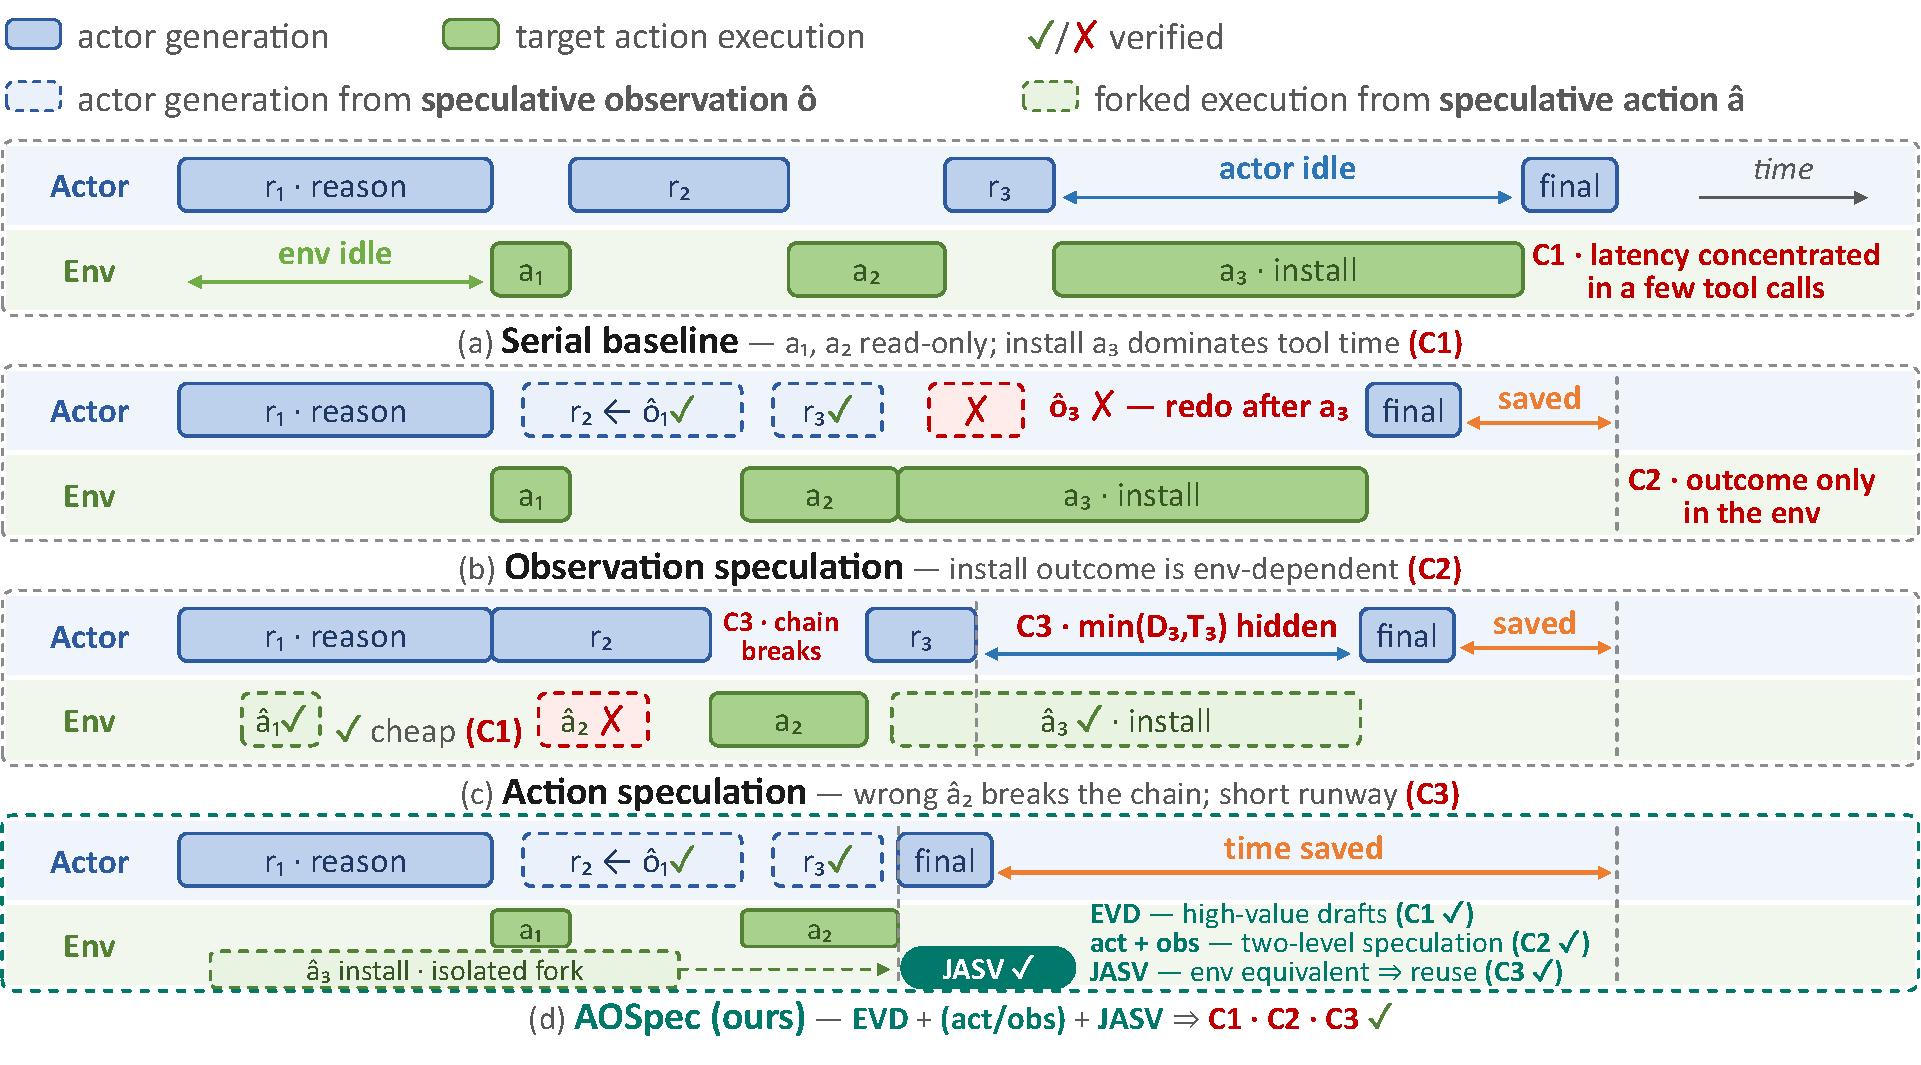
\includegraphics[width=\linewidth]{figs/diagram_v4.pdf}
    \caption{Overview of \sysname{} on a representative agentic trajectory. (a) Serial execution exposes tool latency. (b) Observation only speculation advances predictable outputs but cannot infer environment dependent results. (c) Action only speculation offers little same step overlap and fragile exact chain lookahead. (d) \sysname{} drafts observation with EVD and combines them with isolated target action lookahead, verifying action forks with JASV.}
    \label{fig:method-overview}
\end{figure*}

\section{Methodology}
\label{sec:method}

\subsection{Algorithm Overview}
\label{subsec:overview}

\sysname{} addresses the three requirements identified in Section~\ref{sec:motivation}:
prioritize latency over hit rate, combine predicted and environment-produced observations,
and extend action overlap without predicting an entire future trajectory.
Figure~\ref{fig:method-overview} illustrates how \sysname{} resolves the identified challenges.

At each verified observation boundary, the actor begins generating next action while speculative
actions are launched in isolated sandbox forks. Speculative candidates may target the current or a
later window. When the actor emits the target action $a$, \emph{Joint Action--State Verification} (JASV)
selects a fork only if both the speculative action matches the target action and the original environment matches the committed environment; otherwise, $a$
executes from the committed environment.

A completed action supplies its actual observation immediately. While execution remains
pending, \emph{Expected Value Decoding} (EVD) drafts candidate observations, each of which may start a provisional
actor continuation. When the actual observation returns, only the continuation whose draft is identical to the actual observation is kept. The resulting environment is then committed, and invalid forks
are pruned. Algorithm~\ref{alg:overview} summarizes the control
flow of \sysname{}.

\begin{algorithm}[t]
\caption{\sysname{}: Action--Observation Co-Speculation}
\label{alg:overview}
\small
\begin{algorithmic}[1]
\STATE $H,S\gets$ verified history and committed environment
\STATE $B\gets\textsc{StartActor}(H)$
\STATE $\mathcal F\gets\textsc{LaunchActions}(H,S)$
\WHILE{\textbf{true}}
  \STATE $x\gets\textsc{FinishActor}(B)$
  \IF{$x$ is a terminal response}
    \STATE \textbf{return} $x$
  \ENDIF
  \STATE $a\gets x$
  \STATE $f\gets$ a fork in $\mathcal F$ satisfying
         $\textsc{VerifyAction}(f,a,S)$, if one exists
  \IF{no such $f$ exists}
    \STATE $f\gets\textsc{Execute}(S,a)$
  \ENDIF

  \STATE $\mathcal P\gets\varnothing$
  \IF{$f$ has not finished}
    \STATE Start $\textsc{PredictObservations}(H,a)$
    \FOR{each candidate $\hat o$ that finishes before $f$}
      \STATE $\mathcal P[\hat o]\gets
             \textsc{StartActor}(H\circ(a,\hat o))$
    \ENDFOR
  \ENDIF
  \STATE $(o,S^+)\gets\textsc{Wait}(f)$

  \IF{$o\in\operatorname{dom}(\mathcal P)$}
    \STATE $B'\gets\mathcal P[o]$
  \ELSE
    \STATE $B'\gets\textsc{StartActor}(H\circ(a,o))$
  \ENDIF
  \STATE Cancel unfinished drafts and discard all provisional branches except $B'$

  \STATE $H\gets H\circ(a,o)$; $S\gets\textsc{Commit}(S^+)$
  \STATE $\mathcal F\gets
    \textsc{PruneInvalid}(\mathcal F\setminus\{f\},S)
    \cup\textsc{LaunchActions}(H,S)$
  \STATE $B\gets B'$
\ENDWHILE
\end{algorithmic}
\end{algorithm}

\subsection{Speculative Observation}
\label{subsec:evd}

While action execution remains pending, observation speculation advances actor
generation. Because a small fraction of calls contains most tool time
(Section~\ref{sec:challenge1}), it targets expected time hidden rather than hit rate.

\subsubsection{Optional Observation-Model Fine-Tuning}

Observation-model training could improve accuracy at smaller model sizes and candidate widths, reducing the compute required for drafting. 
Given verified history $H_t$,
action $a_t$, and observation $o_t$, we fine-tune a small model by minimizing
\begin{equation}
\mathcal{L}_{\mathrm{obs}}(\theta)
=
-\sum_{(H_t,a_t,o_t)\in\mathcal D}
\log p_\theta(o\mid H_t,a_t).
\end{equation}
We oversample costly windows to retain rare, latency-critical outcomes.
Execution traces provide supervision directly, without manual labels or
observation classes.

\subsubsection{Expected Value Decoding}

\evd{} separates observation probability from tool time. Given $(H_t,a_t)$, it constructs
a candidate set $\mathcal C(H_t,a_t)$ using one or more proposal mechanisms and estimates
each candidate's associated tool time from historical executions
$\{(o_j,\ttime_j)\}$:
\begin{equation}
\widehat T(c)
=
\frac{\sum_j K(c,o_j)\,\ttime_j}
     {\sum_j K(c,o_j)},
\end{equation}
where $K$ measures outcome similarity. Candidates are ranked by
\begin{equation}
V_o(c)
=
p_\theta(c\mid H_t,a_t)\,\widehat T(c),
\end{equation}
a proxy for expected tool time hidden. The highest-scoring candidates are drafted subject
to the branch budget. $K$ may compare discrete outcome forms or learned representations;
it affects ranking but not verification.

Observation decoding races action execution. Unfinished drafts are cancelled if execution
finishes first; a draft that finishes first starts provisional target-model generation
for step $t+1$. EVD selects what to draft, while the race determines the realized saving.

\subsubsection{Observation Verification}

When execution returns $o_t$, \sysname{} retains only a continuation whose predicted
observation is byte-identical to $o_t$. Mismatching continuations and their descendants
are discarded; if none matches, generation restarts from $o_t$. Canonicalizing
inconsequential fields such as process UUIDs could improve acceptance without changing
application-level semantics.

\subsection{Speculative Action}
\label{subsec:speculative-action}

Observation prediction cannot recover outcomes determined by the execution environment
(Section~\ref{sec:challenge2}). Speculative action instead executes speculative,
latency-critical actions in isolated forks, obtaining their actual observations while
containing their effects. JASV verifies each speculative action and its original environment
before reuse.

\subsubsection{Joint Action--State Verification}
\label{subsec:action-verification}
Each fork $f$ records its speculative action $\hat a_f$ and the version $\nu(S_f)$ of its
original environment. When the actor emits the target $a_i$ from the committed environment $S_i$,
JASV accepts the fork only if both actions and pre-execution environments match:
\begin{equation}
\mathrm{ValidAct}(f,a_i,S_i)
=
[\hat a_f=a_i]
\land
[\nu(S_f)=\nu(S_i)].
\end{equation}
Action equality covers the tool and its arguments. A valid fork executed the same action
from the same environment, so its observation and effects can be reused; otherwise, it
is discarded and $a_i$ executes from $S_i$.

JASV replaces explicit dependency analysis by discarding outstanding speculative forks upon commit. By performing speculative execution within the isolated fork, \sysname{}'s execution is semantically identical to the serial execution, making it a lossless speculation.
In Algorithm~\ref{alg:overview}, $\textsc{PruneInvalid}$ removes stale forks after each
commit, and $\textsc{VerifyAction}$ checks the action and version before reuse.

\subsubsection{State-Verified Action Lookahead}
\label{subsec:action-lookahead}

Longer lookahead increases overlap, but conventionally requires a longer chain of correct
predictions, whose acceptance probability decreases multiplicatively with the lookahead depth
(Section~\ref{sec:challenge3}). JASV instead predicts only the latency-critical target
action and later verifies its launch environment.

If an action issued at step $i$ is launched at boundary $j$, its available runway is
\begin{equation}
R_{j,i}
=
\sum_{k=j}^{i}\dtime_k
+
\sum_{k=j}^{i-1}\ttime_k,
\end{equation}
allowing it to hide up to $\min(\ttime_i,R_{j,i})$ of its execution time.

A candidate may launch at any verified boundary and remains valid across intervening
calls that leave the managed environment unchanged. Thus, these calls need not be
predicted, although forecasting a more distant target may remain harder. Calls apparent
from task context may also launch before the first actor step, similar to prefetching
before task execution.

\subsubsection{Runtime Support}

The sandboxed runtime provides snapshot, fork, execute, commit, and discard operations. Our
implementation assigns each sandbox's copy-on-write (CoW) filesystem image an immutable version, which is uniquely identified by its root hash. 
Forks record their origin version, and commit the verified speculative path, reducing JASV to a
version comparison rather than a recursive scan. Non-filesystem inputs and effects are excluded.
%
Our implementation adopts a CoW agent runtime from concurrent work under
anonymous review; we will add its public citation when available.